\newpage

\section{{\tt sodb8}~\label{sec:sodb8_hist}} 
This section exhibits histograms on the EMPv5 data obtained on {\tt sodb8}. 
The detailed description of the base data are from Table~\ref{tab:exp_notes}.

\subsection{ET}

\begin{figure}[hp!]
	\centering
	\subfigure[ET frequency on INC1]{
		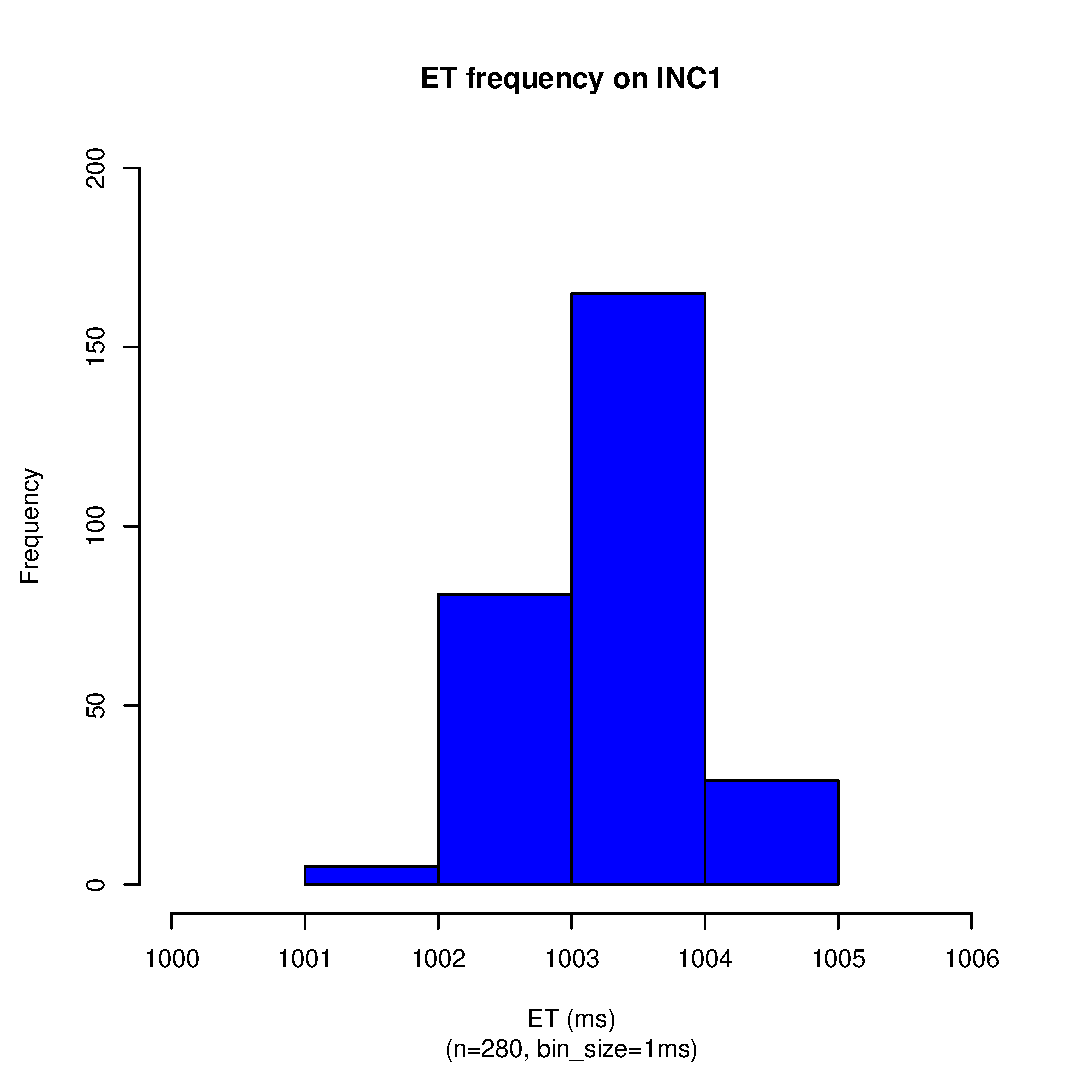
\includegraphics[scale=0.43]{sodb8/1_sec_et_hist_v5.eps}
		\label{fig:inc1_et_hist_v5}
	}
	\subfigure[ET frequency on INC2]{
		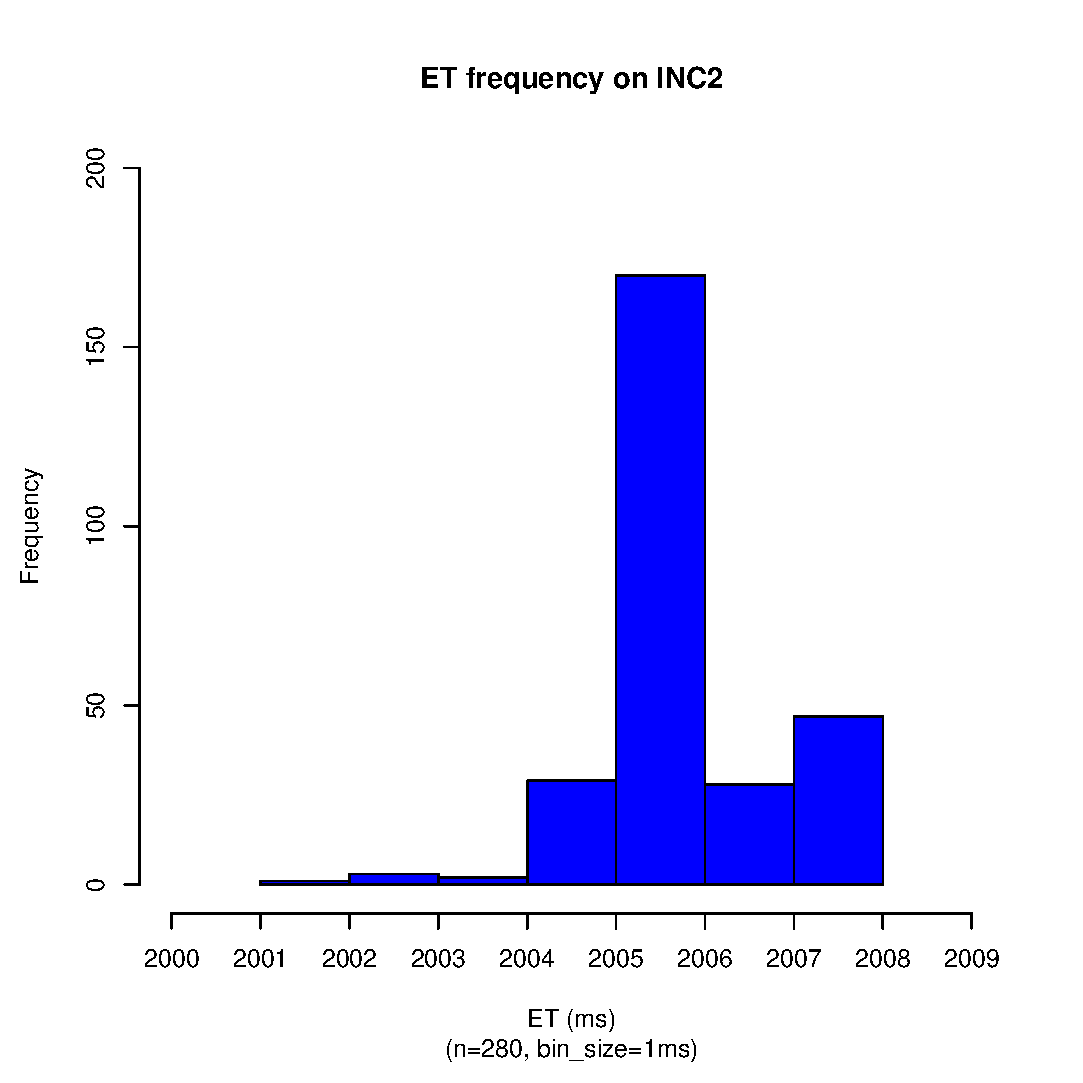
\includegraphics[scale=0.43]{sodb8/2_sec_et_hist_v5.eps}
		\label{fig:inc2_et_hist_v5}
	}
	\subfigure[ET frequency on INC4]{
		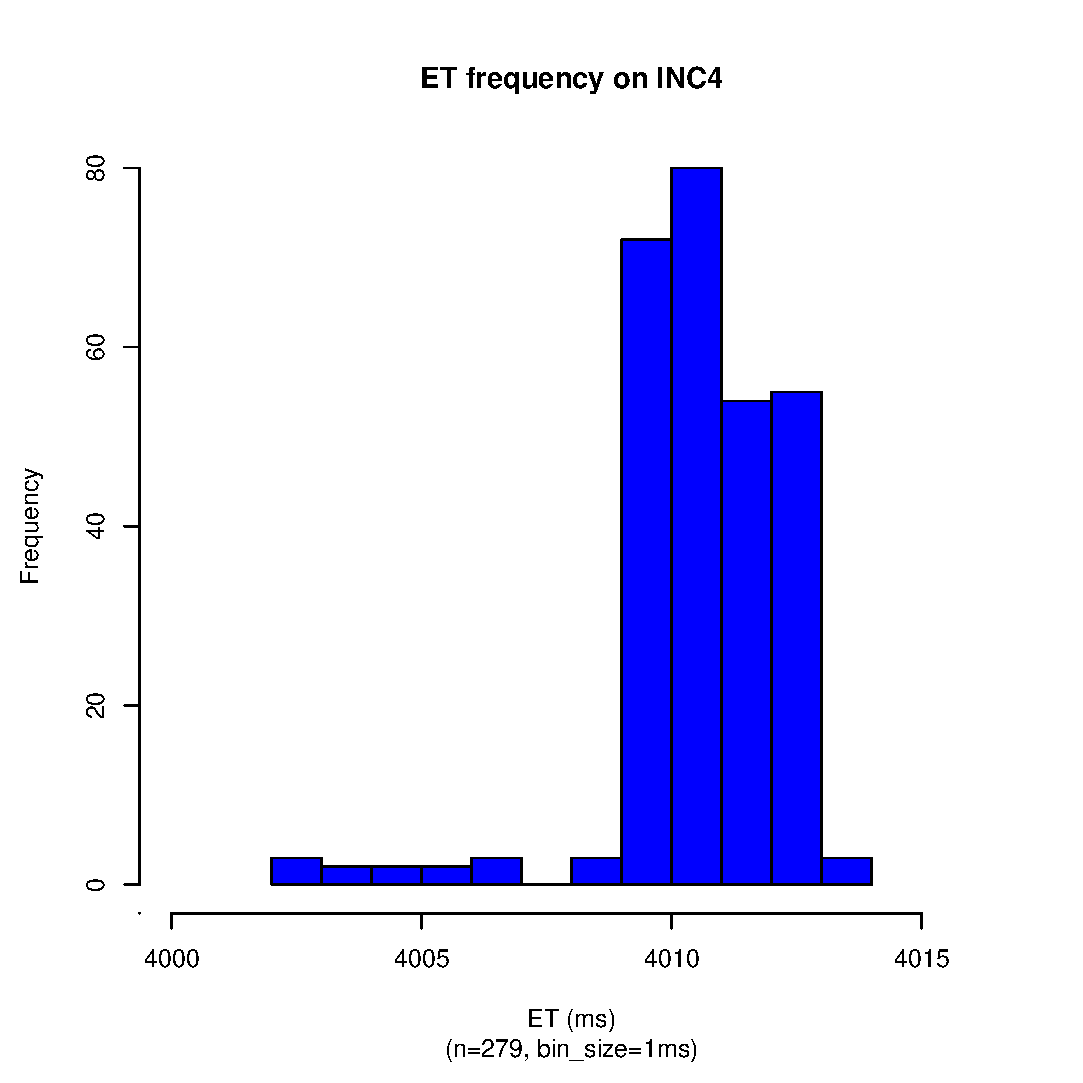
\includegraphics[scale=0.43]{sodb8/4_sec_et_hist_v5.eps}
		\label{fig:inc4_et_hist_v5}
	}
	\subfigure[ET frequency on INC8]{
		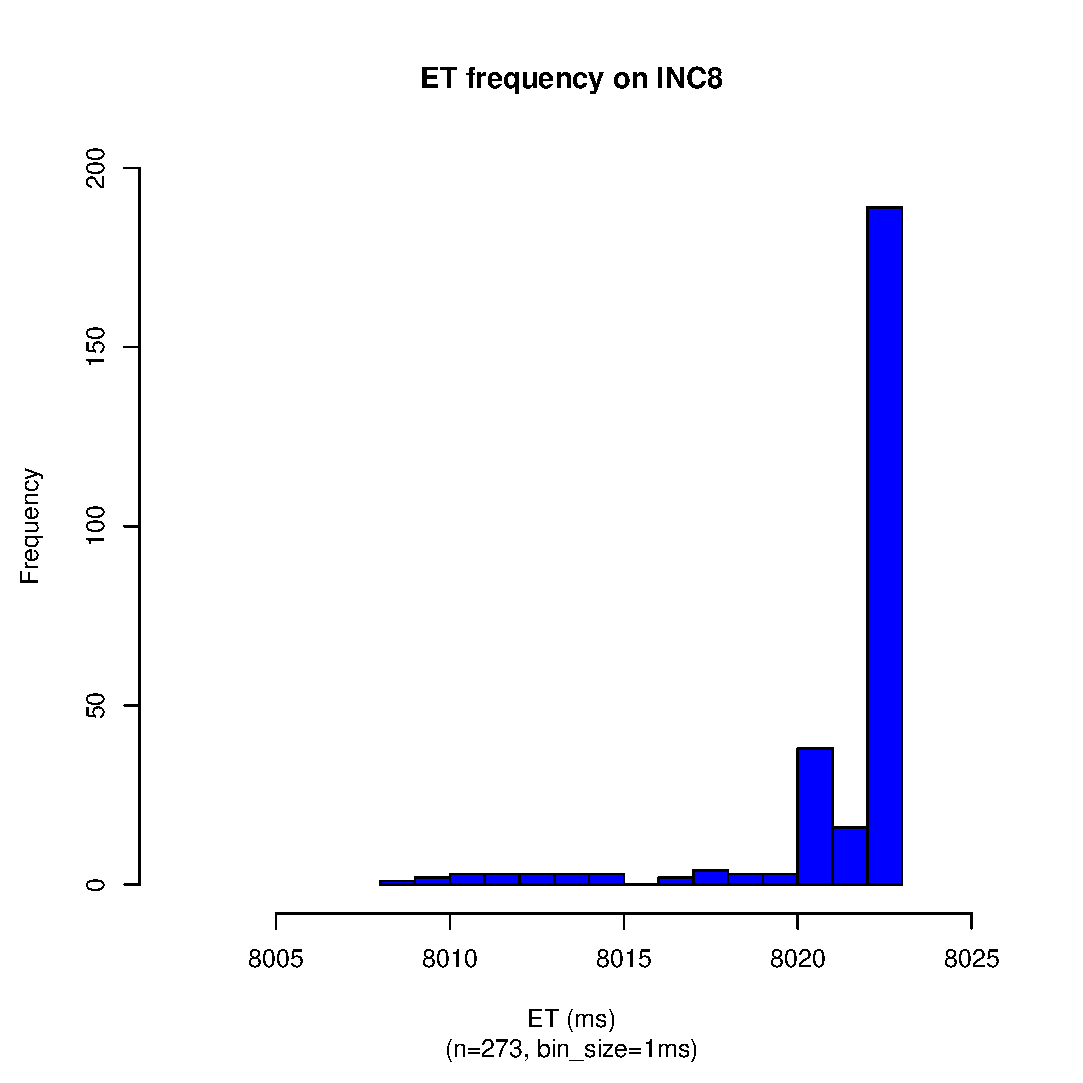
\includegraphics[scale=0.43]{sodb8/8_sec_et_hist_v5.eps}
		\label{fig:inc8_et_hist_v5}
	}
	\caption{ET Histograms of INC1 ... INC8~\label{fig:s8_et_hist1}}
\end{figure}

\begin{figure}[hp!]
	\centering
	\subfigure[ET frequency on INC16]{
		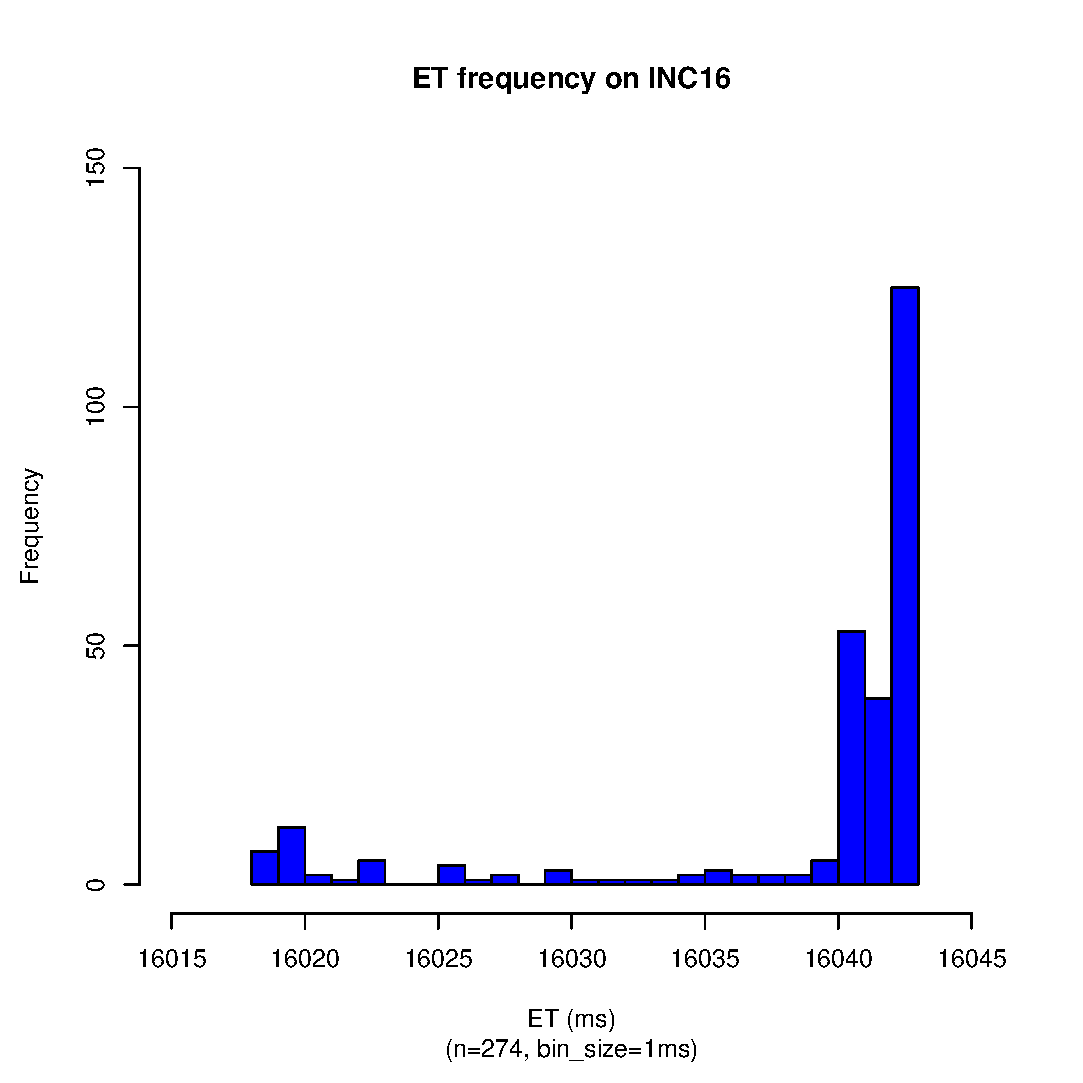
\includegraphics[scale=0.43]{sodb8/16_sec_et_hist_v5.eps}
		\label{fig:inc16_et_hist_v5}
	}
	\subfigure[ET frequency on INC32]{
		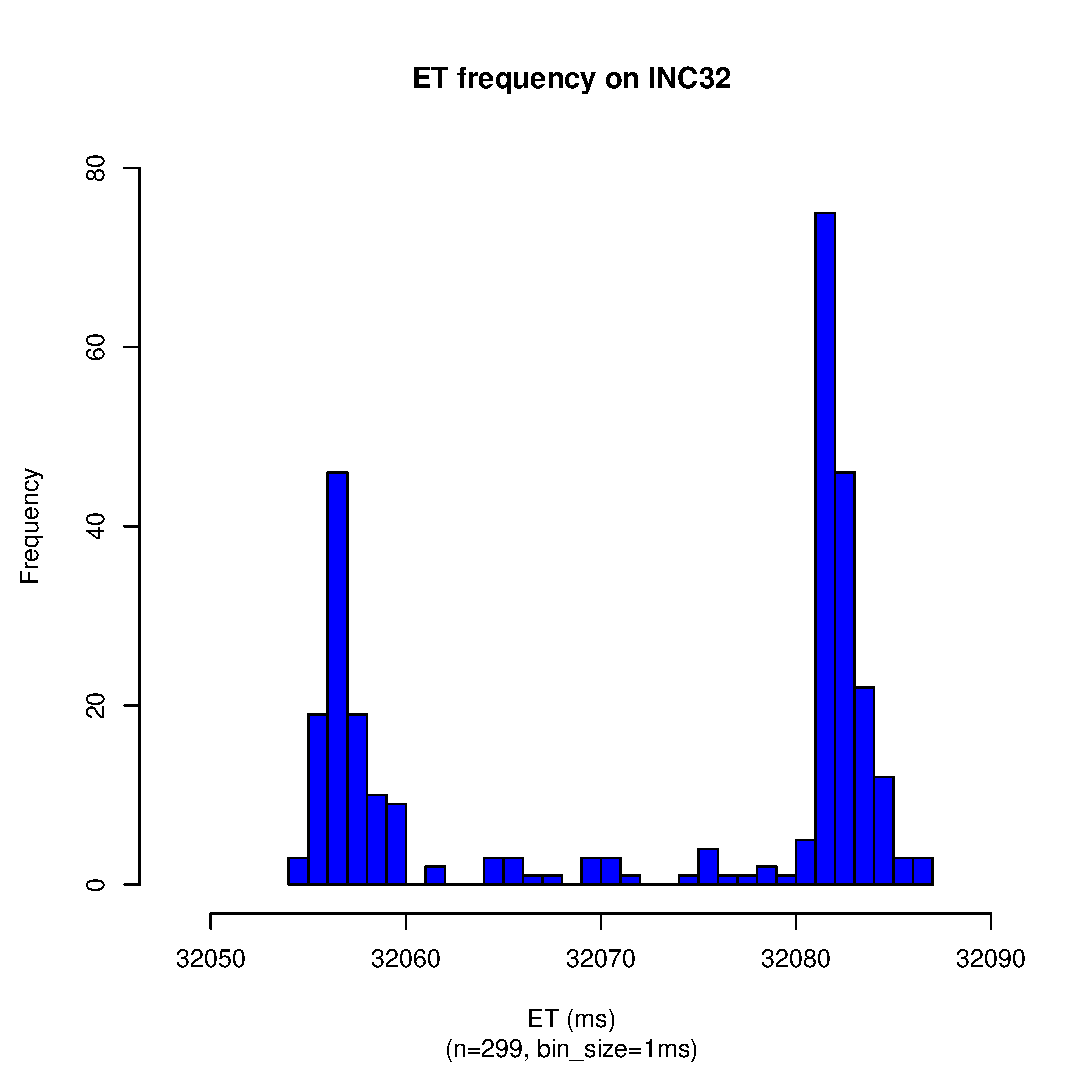
\includegraphics[scale=0.43]{sodb8/32_sec_et_hist_v5.eps}
		\label{fig:inc32_et_hist_v5}
	}
	\subfigure[ET frequency on INC64]{
		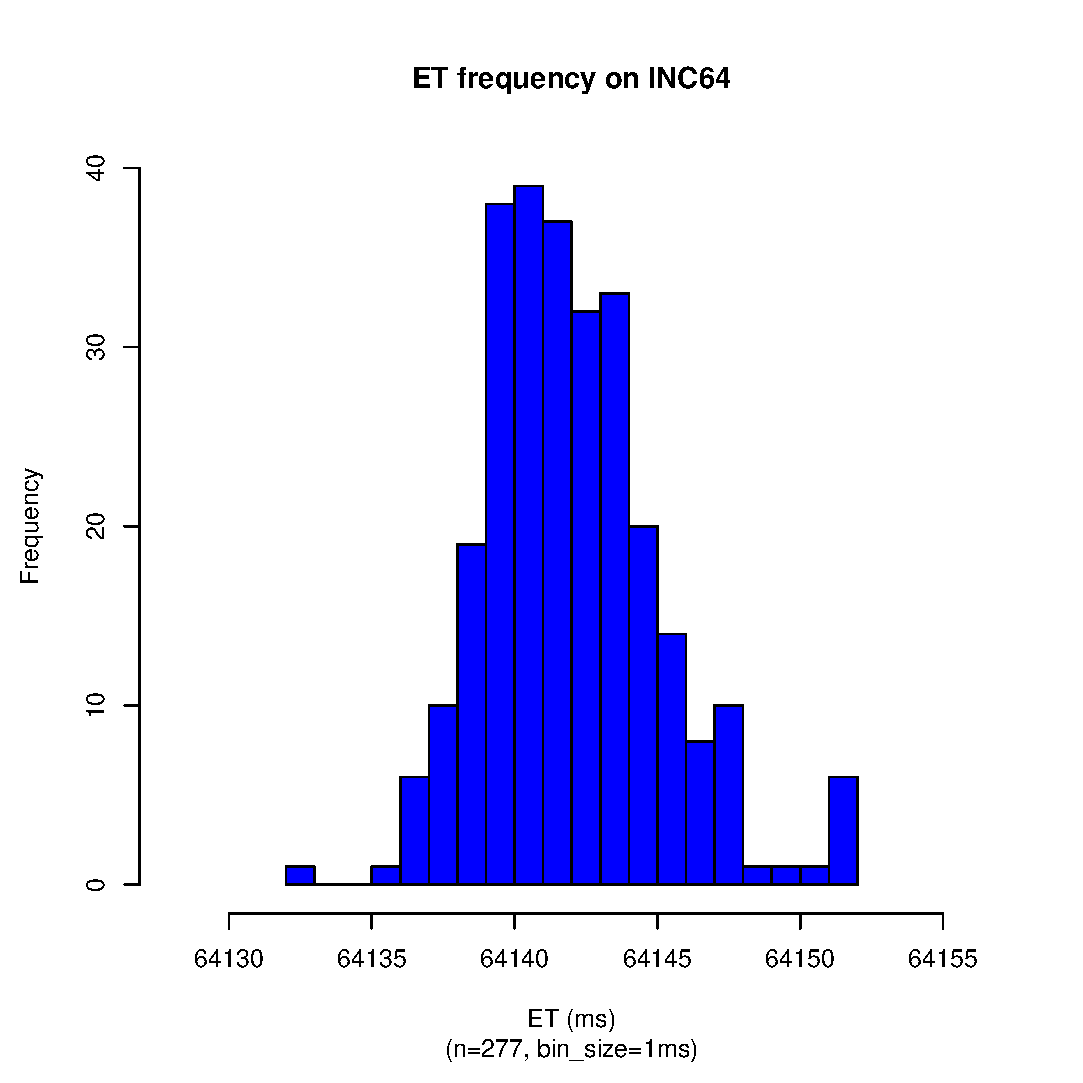
\includegraphics[scale=0.43]{sodb8/64_sec_et_hist_v5.eps}
		\label{fig:inc64_et_hist_v5}
	}
	\subfigure[ET frequency on INC128]{
		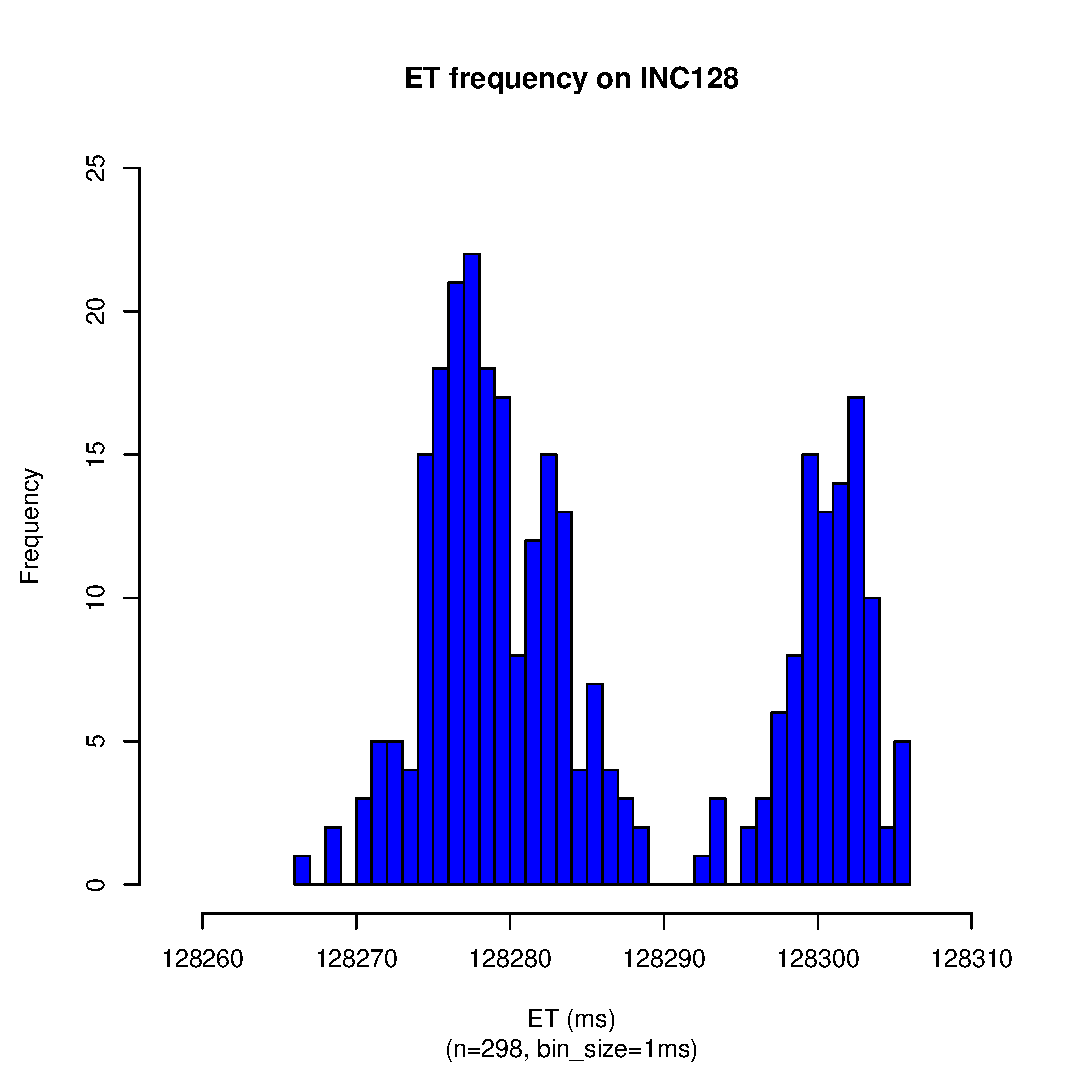
\includegraphics[scale=0.43]{sodb8/128_sec_et_hist_v5.eps}
		\label{fig:inc128_et_hist_v5}
	}
	\caption{ET Histograms of INC16 ... INC128~\label{fig:s8_et_hist2}}
\end{figure}

\newpage

\subsection{PT}

\begin{figure}[hp!]
	\centering
	\subfigure[PT frequency on INC1]{
		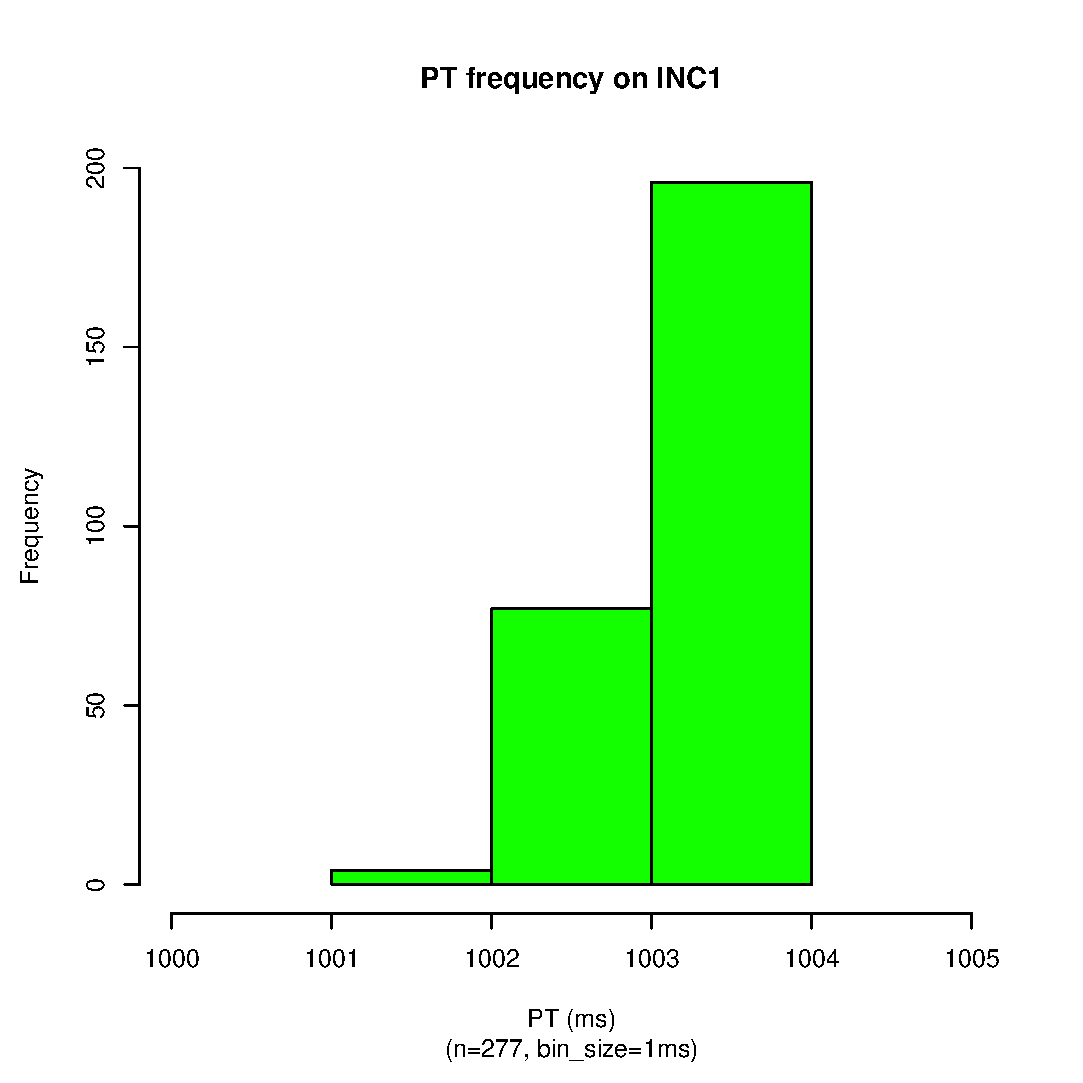
\includegraphics[scale=0.43]{sodb8/1_sec_pt_hist_v5.eps}
		\label{fig:inc1_hist_v5}
	}
	\subfigure[PT frequency on INC2]{
		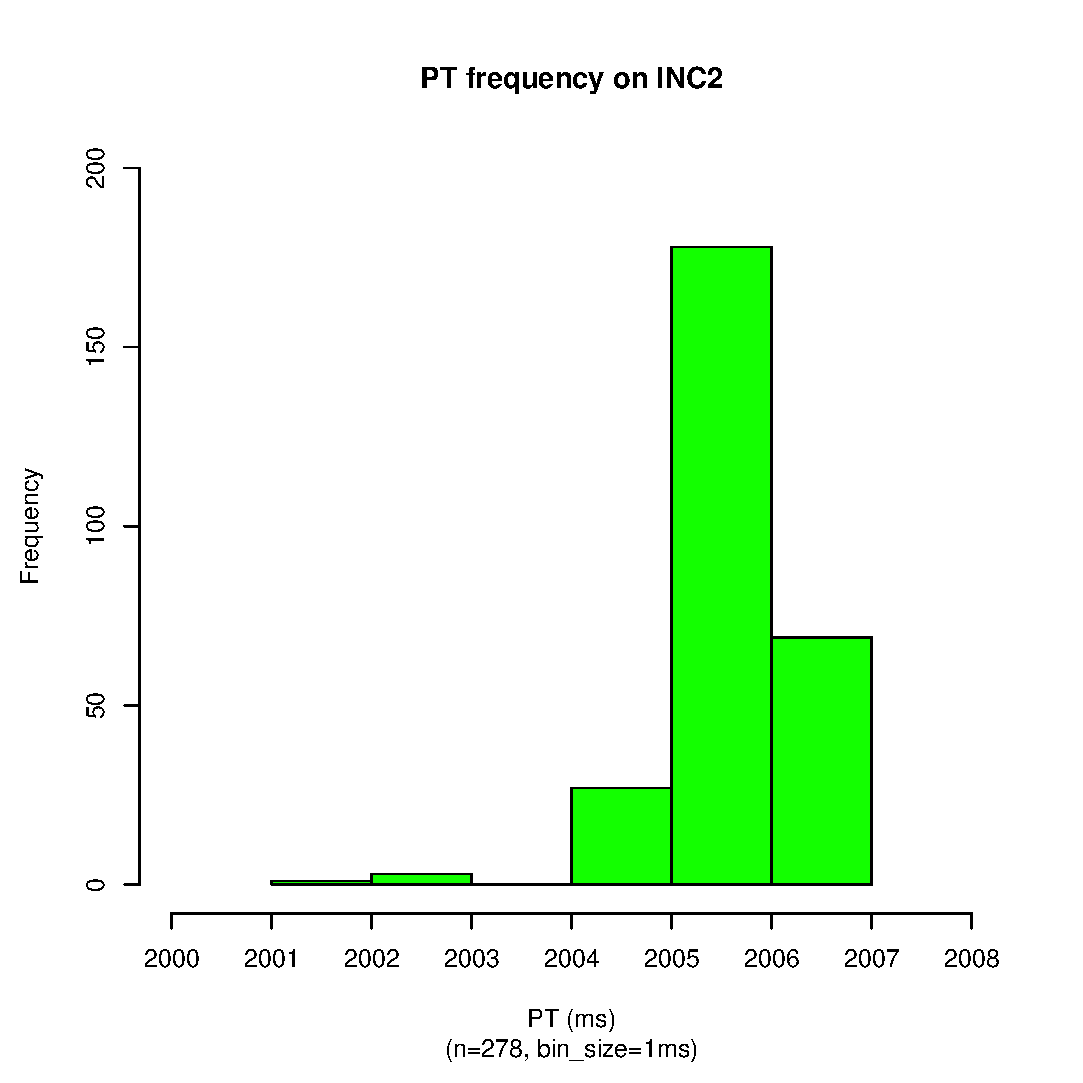
\includegraphics[scale=0.43]{sodb8/2_sec_pt_hist_v5.eps}
		\label{fig:inc2_hist_v5}
	}
	\subfigure[PT frequency on INC4]{
		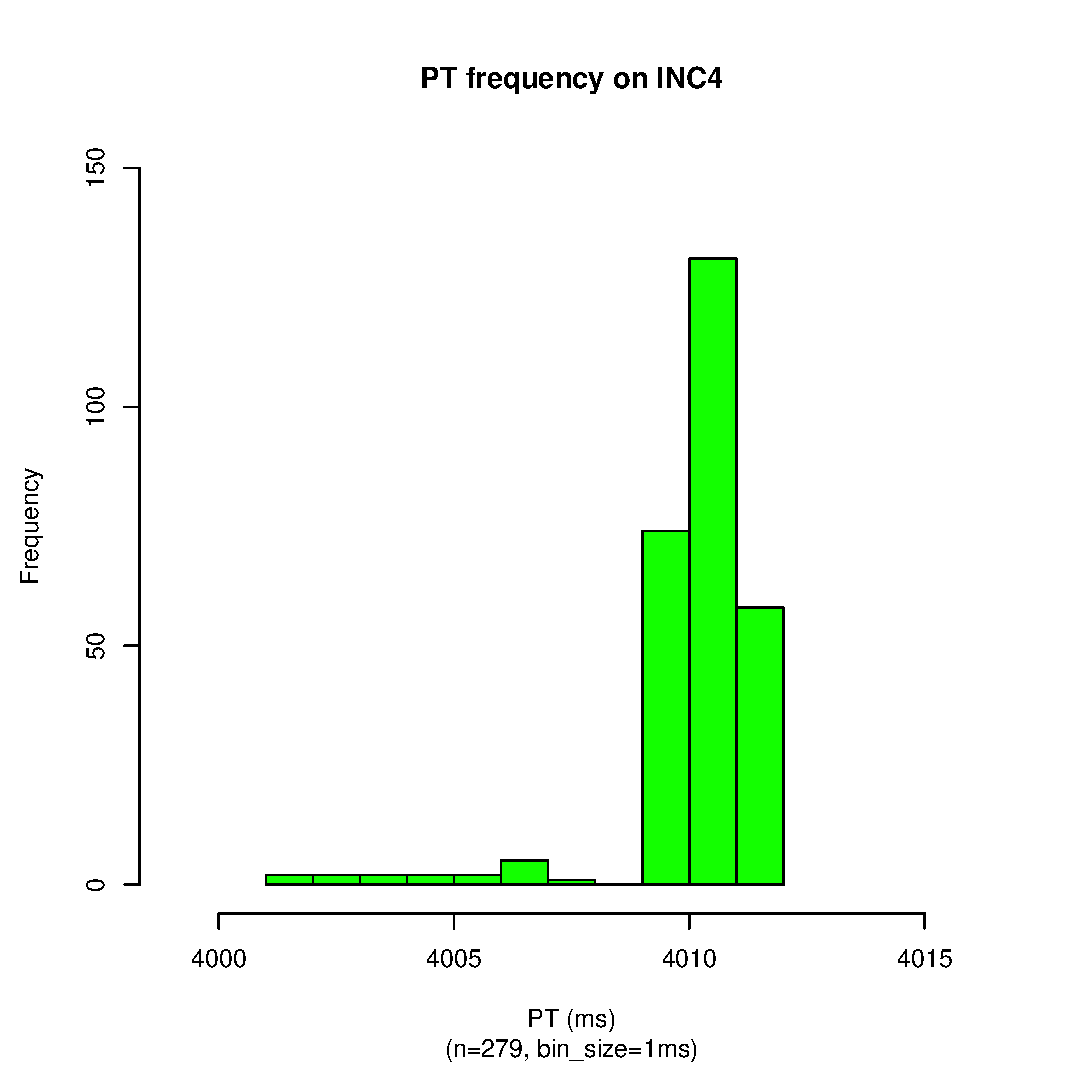
\includegraphics[scale=0.43]{sodb8/4_sec_pt_hist_v5.eps}
		\label{fig:inc4_hist_v5}
	}
	\subfigure[PT frequency on INC8]{
		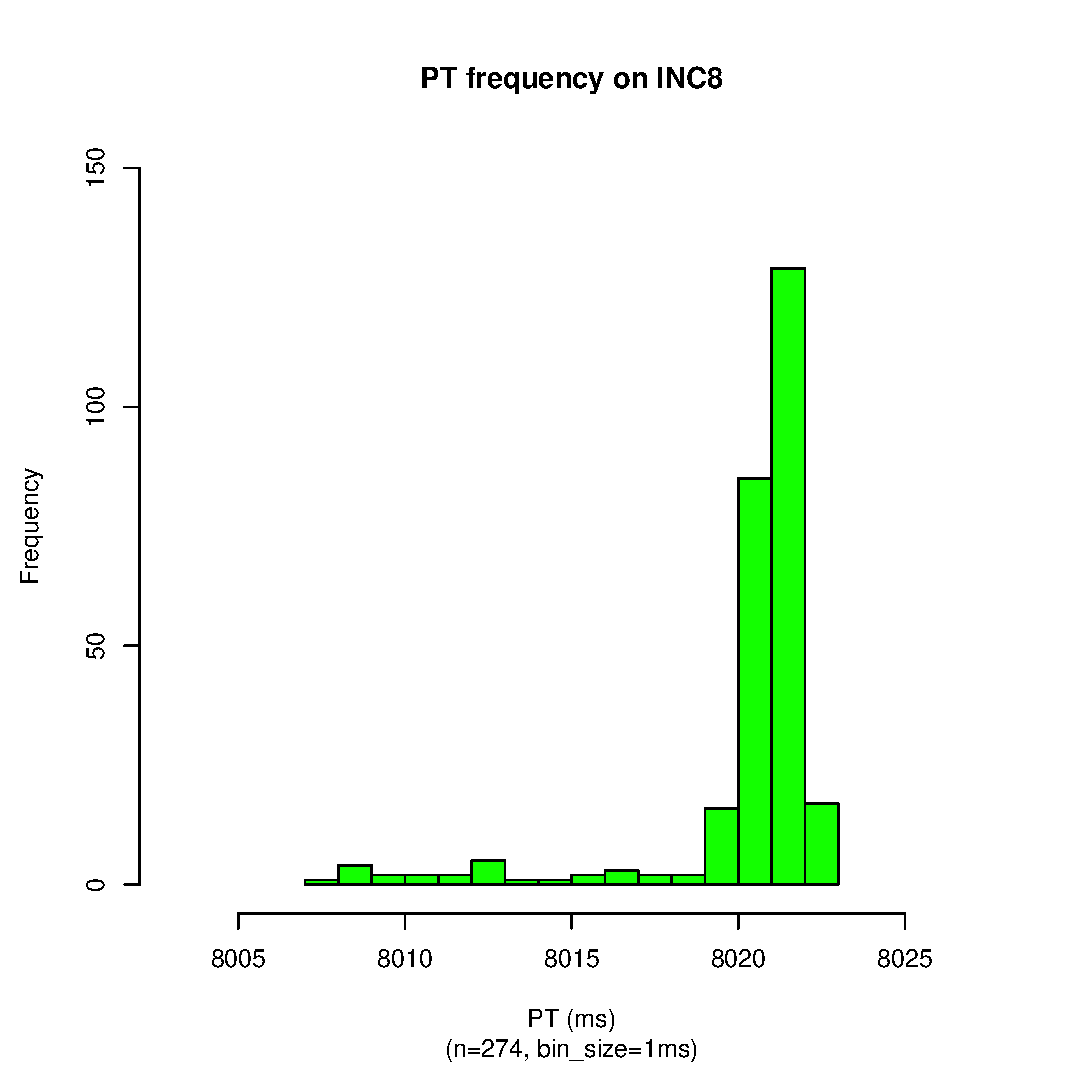
\includegraphics[scale=0.43]{sodb8/8_sec_pt_hist_v5.eps}
		\label{fig:inc8_hist_v5}
	}
	\caption{PT Histograms of INC1 ... INC8~\label{fig:s8_pt_hist1}}
\end{figure}

\begin{figure}[hp!]
	\centering
	\subfigure[PT frequency on INC16]{
		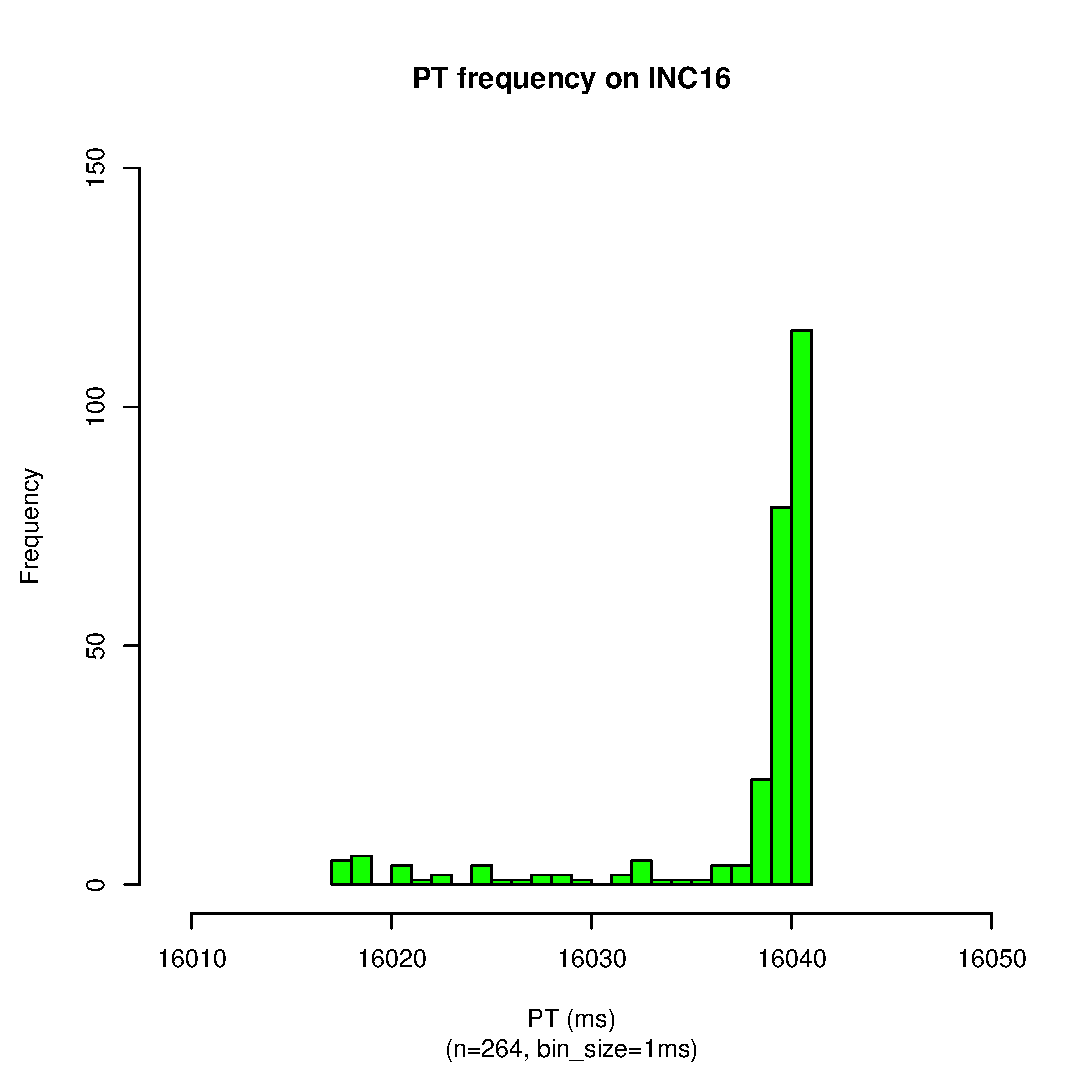
\includegraphics[scale=0.43]{sodb8/16_sec_pt_hist_v5.eps}
		\label{fig:inc16_hist_v5}
	}
	\subfigure[PT frequency on INC32]{
		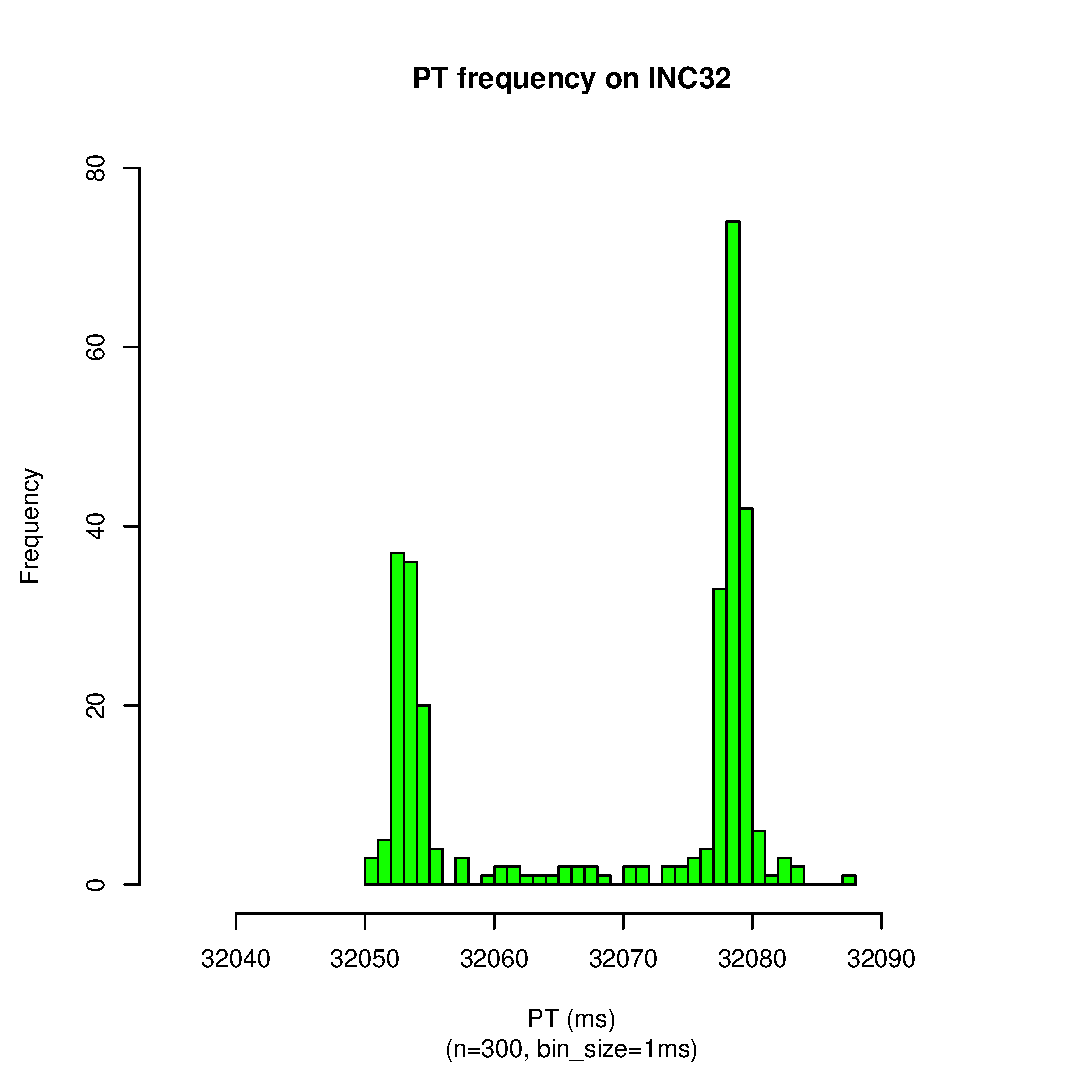
\includegraphics[scale=0.43]{sodb8/32_sec_pt_hist_v5.eps}
		\label{fig:inc32_hist_v5}
	}
	\subfigure[PT frequency on INC64]{
		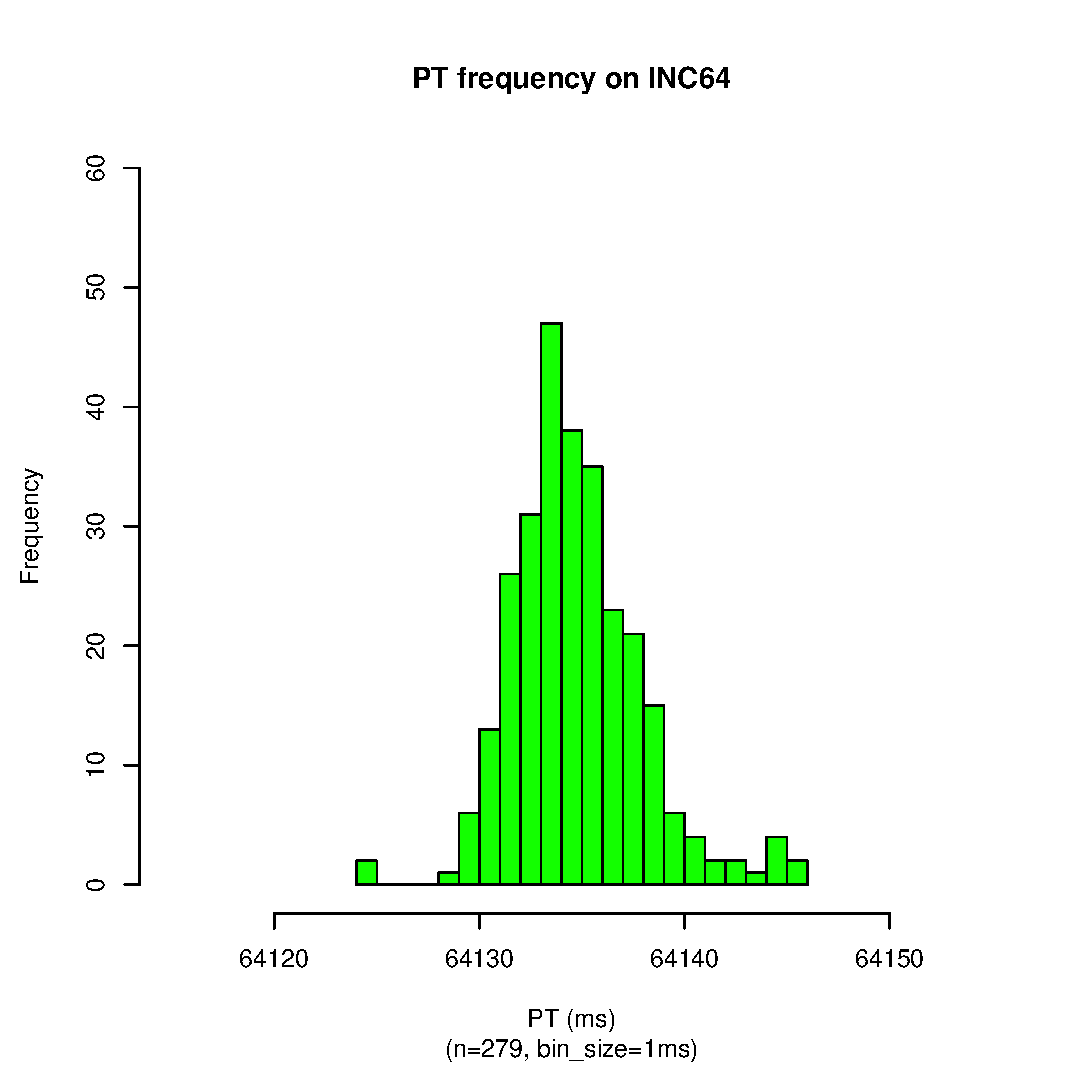
\includegraphics[scale=0.43]{sodb8/64_sec_pt_hist_v5.eps}
		\label{fig:inc64_hist_v5}
	}
	\subfigure[PT frequency on INC128]{
		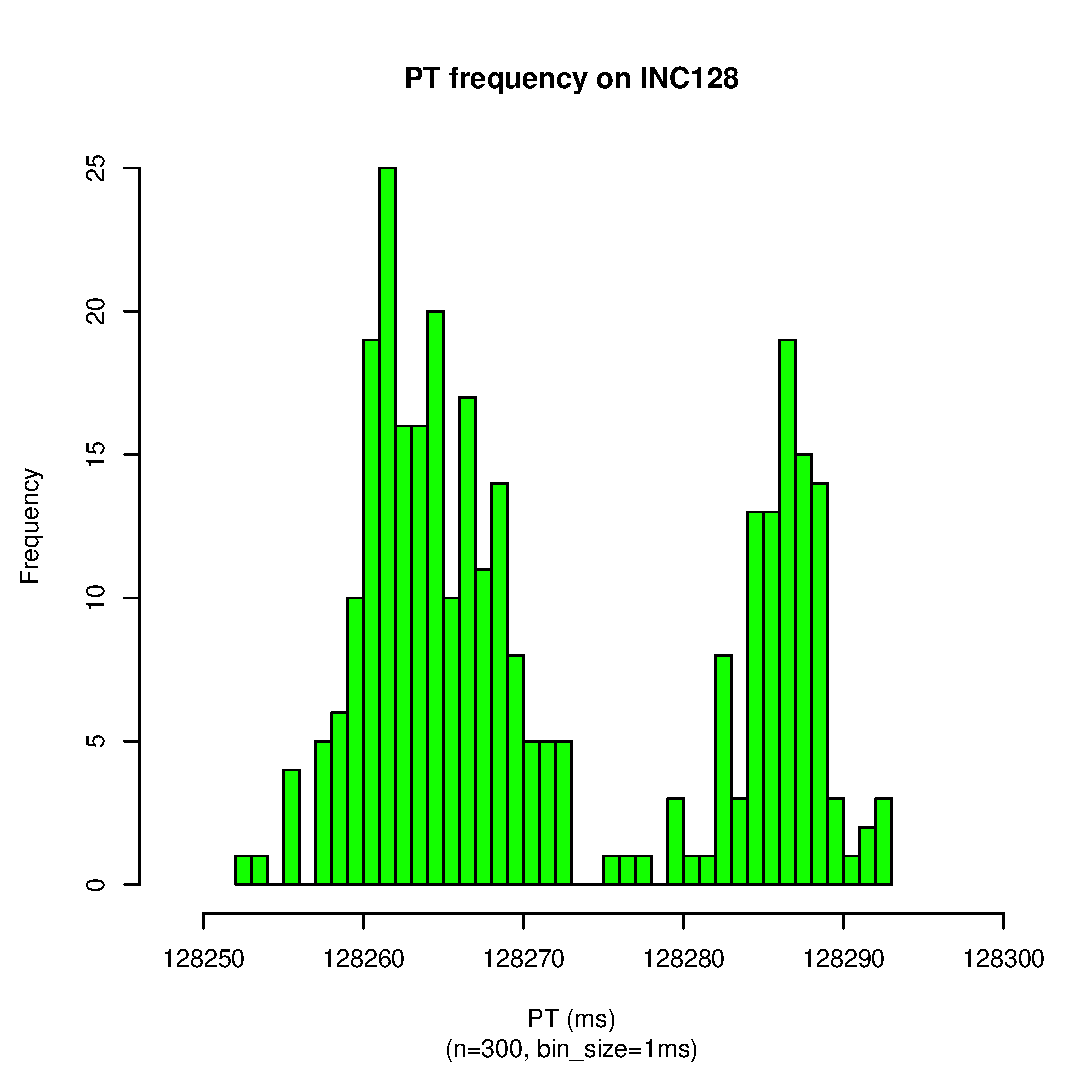
\includegraphics[scale=0.43]{sodb8/128_sec_pt_hist_v5.eps}
		\label{fig:inc128_hist_v5}
	}
	\caption{PT Histograms of INC16 ... INC64~\label{fig:s8_pt_hist2}}
\end{figure}